\appendix

\section{Worst Case Configuration}
\label{sec:appendix-worst-case}
\figref{fig:worst-case} illustrates the worst-case configuration for DeltaSort. This occurs when all updated values cluster at the two ends of the array, forming a single spanning segment. In this case, all left-moving values must be shifted to the left end, and all right-moving values to the right end, resulting in maximum data movement of $O(kn)$.

% Figure: DeltaSort worst-case movement diagram
\begin{figure}[h]
\centering
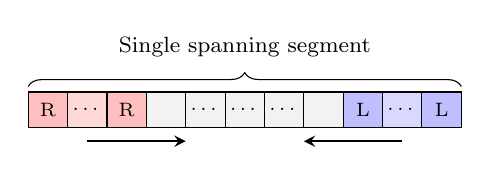
\begin{tikzpicture}[
    cell/.style={minimum width=0.5cm, minimum height=0.45cm, draw, font=\scriptsize, inner sep=0pt, outer sep=0pt, anchor=center},
    right/.style={cell, fill=red!25},
    left/.style={cell, fill=blue!25},
    clean/.style={cell, fill=gray!10, font=\scriptsize},
    segbrace/.style={decorate, decoration={brace, amplitude=5pt}},
    seglabel/.style={font=\footnotesize},
]

\def\yarr{0}
\def\cellw{0.5}

% Place cells at exact positions (center anchored, spaced by cellw)
\node[right] (c0) at (0*\cellw, \yarr) {R};
\node[cell, fill=red!15] (c1) at (1*\cellw, \yarr) {\dots};
\node[right] (c2) at (2*\cellw, \yarr) {R};
\node[clean] (c3) at (3*\cellw, \yarr) {};
\node[cell, fill=gray!10] (c4) at (4*\cellw, \yarr) {\dots};
\node[cell, fill=gray!10] (c5) at (5*\cellw, \yarr) {\dots};
\node[cell, fill=gray!10] (c6) at (6*\cellw, \yarr) {\dots};
\node[clean] (c7) at (7*\cellw, \yarr) {};
\node[left] (c8) at (8*\cellw, \yarr) {L};
\node[cell, fill=blue!15] (c9) at (9*\cellw, \yarr) {\dots};
\node[left] (c10) at (10*\cellw, \yarr) {L};

% Brace spanning entire array
\draw[segbrace] ([yshift=2pt]c0.north west) -- ([yshift=2pt]c10.north east);
\node[seglabel] at (5*\cellw, 0.8) {Single spanning segment};

% Arrows below showing movement directions
\draw[->, thick, >=stealth] (1*\cellw, -0.4) -- (3.5*\cellw, -0.4);
\draw[->, thick, >=stealth] (9*\cellw, -0.4) -- (6.5*\cellw, -0.4);

\end{tikzpicture}
\caption{Worst-case configuration for DeltaSort is formed when updated values cluster at ends of the array and form a single spanning segment.}
\label{fig:worst-case}
\end{figure}


\section{Empirical Validation of Complexity Bounds}
\label{sec:appendix-complexity}

\figref{fig:complexity-analysis} presents empirical validation of DeltaSort's complexity bounds across multiple scales of $n$ and $k$. For movement complexity, we normalize the measured movement by $n\sqrt{k}$; for comparison complexity, we normalize by $k\log n$. If the theoretical bounds are tight, these normalised values should be approximately constant across all scales.

The results confirm both bounds: movement normalised by $n\sqrt{k}$ converges to approximately $0.4$ across four orders of magnitude of $n$, and comparisons normalised by $k\log n$ converge to approximately $2$. The overlap of lines for different $n$ values validates that the asymptotic analysis correctly captures the algorithm's behavior.

% Figure: Empirical validation of complexity bounds
% Movement: O(n√k) → normalized = movement / (n√k) should be constant
% Comparisons: O(k log n) → normalized = comparisons / (k log n) should be constant
\begin{figure}[t]
\centering
\begin{minipage}{0.48\textwidth}
\centering
\begin{tikzpicture}
\begin{axis}[
    width=\textwidth,
    height=5.5cm,
    xlabel={$k$ (\% of $n$)},
    ylabel={Movement / $(n\sqrt{k})$},
    xmode=log,
    log basis x=10,
    xmin=0.08, xmax=25,
    ymin=0, ymax=0.6,
    xtick={0.1, 1, 10},
    xticklabels={0.1, 1, 10},
    grid=both,
    grid style={line width=0.1pt, draw=gray!30},
    major grid style={line width=0.2pt, draw=gray!50},
    legend style={font=\footnotesize, at={(0.98,0.02)}, anchor=south east},
    title={\textbf{(a) Normalized Movement}},
]

% n = 1K
\addplot[color=blue!70, mark=*, thick, mark size=2pt] 
    table[col sep=comma, x=k_percent, y=movement_normalized, 
          restrict expr to domain={\thisrow{n}}{1000:1000}] {\rootdir/figures/movement-analysis.csv};
\addlegendentry{$n=1$K}

% n = 10K  
\addplot[color=red!70, mark=square*, thick, mark size=2pt]
    table[col sep=comma, x=k_percent, y=movement_normalized,
          restrict expr to domain={\thisrow{n}}{10000:10000}] {\rootdir/figures/movement-analysis.csv};
\addlegendentry{$n=10$K}

% n = 100K
\addplot[color=green!60!black, mark=triangle*, thick, mark size=2pt]
    table[col sep=comma, x=k_percent, y=movement_normalized,
          restrict expr to domain={\thisrow{n}}{100000:100000}] {\rootdir/figures/movement-analysis.csv};
\addlegendentry{$n=100$K}

% n = 1M
\addplot[color=purple!70, mark=diamond*, thick, mark size=2pt]
    table[col sep=comma, x=k_percent, y=movement_normalized,
          restrict expr to domain={\thisrow{n}}{1000000:1000000}] {\rootdir/figures/movement-analysis.csv};
\addlegendentry{$n=1$M}

\end{axis}
\end{tikzpicture}
\end{minipage}%
\hfill%
\begin{minipage}{0.48\textwidth}
\centering
\begin{tikzpicture}
\begin{axis}[
    width=\textwidth,
    height=5.5cm,
    xlabel={$k$ (\% of $n$)},
    ylabel={Comparisons / $(k \log (n\sqrt{k}))$},
    xmode=log,
    log basis x=10,
    xmin=0.08, xmax=25,
    ymin=0, ymax=2,
    xtick={0.1, 1, 10},
    xticklabels={0.1, 1, 10},
    grid=both,
    grid style={line width=0.1pt, draw=gray!30},
    major grid style={line width=0.2pt, draw=gray!50},
    legend style={font=\footnotesize, at={(0.98,0.02)}, anchor=south east},
    title={\textbf{(b) Normalized Comparisons}},
]

% n = 1K
\addplot[color=blue!70, mark=*, thick, mark size=2pt] 
    table[col sep=comma, x=k_percent, y=normalized,
          restrict expr to domain={\thisrow{n}}{1000:1000}] {\rootdir/figures/comparator-analysis.csv};
\addlegendentry{$n=1$K}

% n = 10K  
\addplot[color=red!70, mark=square*, thick, mark size=2pt]
    table[col sep=comma, x=k_percent, y=normalized,
          restrict expr to domain={\thisrow{n}}{10000:10000}] {\rootdir/figures/comparator-analysis.csv};
\addlegendentry{$n=10$K}

% n = 100K
\addplot[color=green!60!black, mark=triangle*, thick, mark size=2pt]
    table[col sep=comma, x=k_percent, y=normalized,
          restrict expr to domain={\thisrow{n}}{100000:100000}] {\rootdir/figures/comparator-analysis.csv};
\addlegendentry{$n=100$K}

% n = 1M
\addplot[color=purple!70, mark=diamond*, thick, mark size=2pt]
    table[col sep=comma, x=k_percent, y=normalized,
          restrict expr to domain={\thisrow{n}}{1000000:1000000}] {\rootdir/figures/comparator-analysis.csv};
\addlegendentry{$n=1$M}

\end{axis}
\end{tikzpicture}
\end{minipage}
\caption{Empirical assessment of DeltaSort's complexity bounds. Each line represents a different array size $n$. (a)~Movement normalized by $n\sqrt{k}$ converges to $\approx 0.4$, confirming $O(n\sqrt{k})$. (b)~Comparisons normalized by $k\log (n\sqrt{k})$ converges to $\approx 1.4$, confirming $O(k\log (n\sqrt{k}))$. The overlap of lines across scales indicates that the asymptotic bounds are valid.}
\label{fig:complexity-analysis}
\end{figure}


\section{JavaScript/V8 Benchmarks}
\label{sec:appendix-js-deltasort}

% Figure: Combined Rust performance (execution time + crossover)
\begin{figure}[t]
\centering
\begin{minipage}{0.47\textwidth}
\centering
\begin{tikzpicture}
\begin{axis}[
    width=0.95\textwidth,
    height=5.5cm,
    xlabel={Percentage of updated values ($k/n$)},
    ylabel={Execution time (\textmu s)},
    xmode=log,
    ymode=log,
    log basis x=10,
    log basis y=10,
    xmin=1, xmax=100000,
    ymin=5, ymax=100000,
    xtick={1, 10, 100, 1000, 10000, 100000},
    xticklabels={.001\%, .01\%, .1\%, 1\%, 10\%, 100\%},
    ytick pos=left,
    grid=major,
    major grid style={line width=0.3pt, draw=gray!30},
    tick label style={font=\scriptsize},
    label style={font=\small},
    title={\textbf{(a) Execution Time ($n=100$K)}},
    legend to name=rustlegend,
    legend style={font=\scriptsize, legend columns=4, column sep=0.3em},
    clip=false,
]

% Crossover vertical lines (drop lines to x-axis)
\draw[orange!60, densely dashed, line width=0.8pt] (axis cs:39,5) -- (axis cs:39,100000);
\draw[green!50!black, densely dashed, line width=0.8pt] (axis cs:31433,5) -- (axis cs:31433,100000);
\draw[purple!50, densely dashed, line width=0.8pt] (axis cs:76974,5) -- (axis cs:76974,100000);

% Crossover labels (above and left of lines)
\node[font=\tiny, orange!80!black, anchor=south east] at (axis cs:50,4.3) {.04\%};
\node[font=\tiny, green!60!black, anchor=south east] at (axis cs:41433,4.3) {31\%};
\node[font=\tiny, purple!70, anchor=south east] at (axis cs:400974,4.3) {77\%};

% FullSort
\addplot[color=gray!70, mark=square*, thick, mark size=1.5pt] 
    table[col sep=comma, x=k, y=native] {\rootdir/figures/rust/execution-time.csv};

% Binary Insertion
\addplot[color=orange!80, mark=triangle*, thick, mark size=1.5pt] 
    table[col sep=comma, x=k, y=bis] {\rootdir/figures/rust/execution-time.csv};

% Extract-Sort-Merge
\addplot[color=purple!70, mark=diamond*, thick, mark size=1.5pt] 
    table[col sep=comma, x=k, y=esm] {\rootdir/figures/rust/execution-time.csv};

% DeltaSort (emphasized)
\addplot[color=green!70!black, mark=*, thick, mark size=2pt, line width=1.2pt] 
    table[col sep=comma, x=k, y=deltasort] {\rootdir/figures/rust/execution-time.csv};

\legend{FullSort, BIS, ESM, \textbf{DeltaSort}}
\end{axis}
\end{tikzpicture}
\end{minipage}%
\hfill%
\begin{minipage}{0.47\textwidth}
\centering
\begin{tikzpicture}
\begin{axis}[
    width=0.95\textwidth,
    height=5.5cm,
    xlabel={Array size ($n$)},
    ylabel={Crossover $k_c / n$ (\%)},
    xmode=log,
    log basis x=10,
    xmin=1000, xmax=1000000,
    ymin=0, ymax=100,
    ytick={0, 20, 40, 60, 80, 100},
    xtick={1000, 10000, 100000, 1000000},
    xticklabels={1K, 10K, \textbf{100K}, 1M},
    grid=both,
    grid style={line width=0.1pt, draw=gray!20},
    major grid style={line width=0.5pt, draw=gray!40},
    tick label style={font=\scriptsize},
    label style={font=\small},
    title={\textbf{(b) Crossover Threshold}},
]

% Highlight line at n=100K
\draw[gray!40, line width=6pt] (axis cs:100000,0) -- (axis cs:100000,100);

% Crossover markers at n=100K
\node[font=\tiny, orange!80!black, anchor=west] at (axis cs:110000,6) {.04\%};
\node[font=\tiny, green!60!black, anchor=west] at (axis cs:110000,36.5) {31\%};
\node[font=\tiny, purple!70, anchor=west] at (axis cs:110000,77) {77\%};

% BIS crossover
\addplot[color=orange!80, mark=triangle*, thick, mark size=2pt, line width=1.2pt] 
    table[col sep=comma, x=n, y=bis] {\rootdir/figures/rust/crossover-all.csv};

% ESM crossover
\addplot[color=purple!70, mark=diamond*, thick, mark size=2pt, line width=1.2pt] 
    table[col sep=comma, x=n, y=esm] {\rootdir/figures/rust/crossover-all.csv};

% DeltaSort crossover
\addplot[color=green!70!black, mark=*, thick, mark size=2pt, line width=1.5pt] 
    table[col sep=comma, x=n, y=deltasort] {\rootdir/figures/rust/crossover-all.csv};

\end{axis}
\end{tikzpicture}
\end{minipage}

\vspace{0.3em}
\ref{rustlegend}
\caption{Rust benchmark results. (a)~Execution time for $n=100$K on log-log scale. Dashed lines mark crossover points where each algorithm loses to FullSort. (b)~Crossover threshold ($k_c/n$) across scales; the shaded line at $n=100$K corresponds to (a). Refer~\appref{sec:appendix-raw-data} for raw data.}
\label{fig:rust-performance}
\end{figure}


\figref{fig:js-performance} shows execution time and crossover threshold data for JavaScript/V8. Several observations emerge:

\begin{enumerate}
  \item DeltaSort and BIS show almost identical performance profiles. This indicates that \emph{the underlying memory movement cost in V8 is not proportional to the number of moved values}. As a result, DeltaSort's core optimization---reducing physical data movement through segmentation---does not translate into wall-clock improvements. This could be because V8 has different kinds of array representations~\cite{v8elementskinds} that may not guarantee contiguous layouts.
  \item ESM is $\sim 40\%$ faster than FullSort (\texttt{Array.prototype.sort}) for $k$ up to $\approx 50\%$. This indicates that \textbf{even in managed runtimes, we can leverage information of updated indices to unlock better performance}.
\end{enumerate}

The key takeaway is that \emph{DeltaSort's performance benefits rely on a predictable movement cost model}, which holds in low-level, unmanaged environments (e.g., Rust) but not in managed runtimes such as V8. Hence in V8, a valid hybrid strategy can be: use BIS for $k \ll n$, ESM for $k \lesssim 40\%$, \texttt{Array.prototype.sort} for $k \gtrsim 40\%$.
